\documentclass[a0paper, portrait, fontscale=0.255]{baposter}

\usepackage[utf8]{inputenc}
\usepackage[T1]{fontenc}

\usepackage{enumitem}
\usepackage{picins}
\usepackage[sfdefault]{Fira Sans}

\definecolor{blue}{RGB}{0, 190, 255}

\begin{document}

\color{black!80}

\begin{poster}{
    background=plain,
    bgColorOne=black!5,
    columns=2,
    headerborder=none,
    headershape=smallrounded,
    textborder=none,
    headershade=plain,
    boxshade=plain,
    headerColorOne=black!15,
    boxColorOne=white,
    headerFontColor=black
}
{
\includegraphics[height=7em]{logos/mff-black.pdf}}
{Data Preprocessing Strategies in Imbalanced Data Classification}
{\vspace{1ex} Radovan Haluška, Supervisor: prof. RNDr. Tomáš Skopal, Ph.D.}
{
\includegraphics[height=7em]{logos/uk-red.pdf}}


% Left column
\begin{posterbox}[column=0, name=background]{Background}
    \parpic[r][t]{
        \begin{minipage}{0.4\linewidth}
            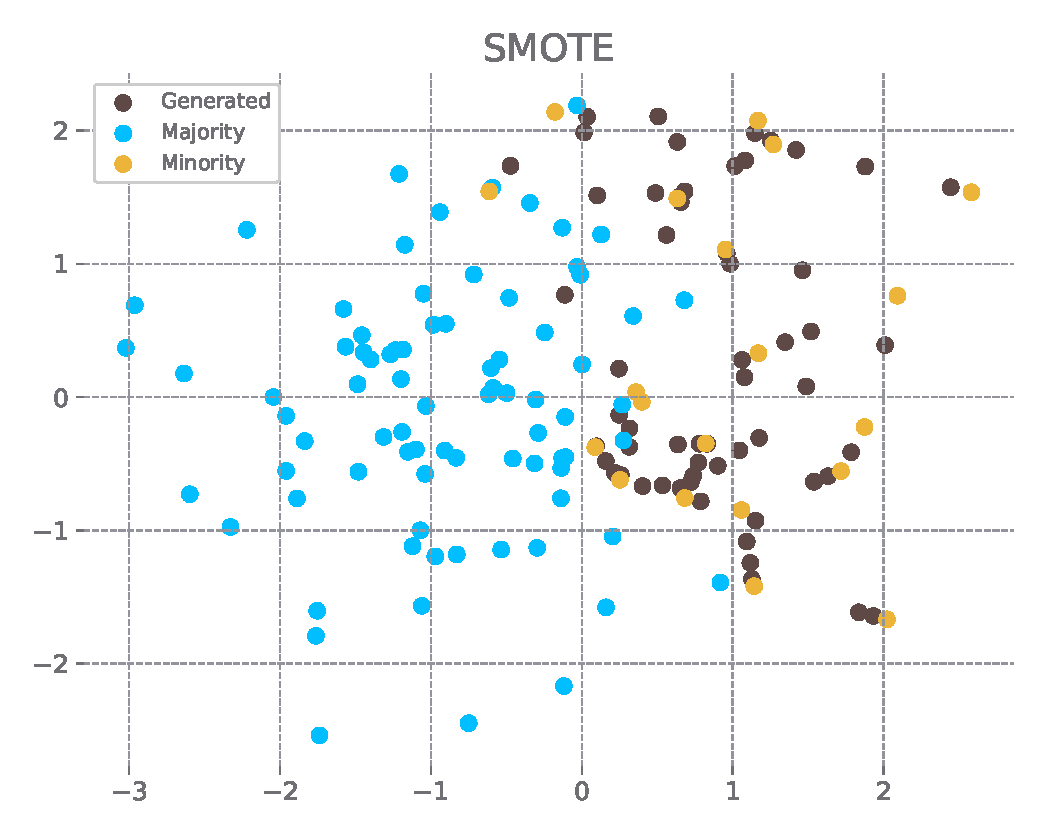
\includegraphics[width=\linewidth]{figures/smote.eps}
        \end{minipage}
    }

    The imbalanced classification problem emerges when the training dataset exhibits an unequal
    distribution between individual classes. Imbalance in training data can severely compromise the
    performance of standard machine learning algorithms, such as decision trees. These classifiers
    expect an approximately balanced distribution of samples into classes. A frequent and least
    invasive approach to dealing with imbalanced datasets is running a preprocessing algorithm
    before training. This thesis aims to benchmark these preprocessing algorithms.

\end{posterbox}


\begin{posterbox}[
    column=0, name=goals, below=background, headerColorOne=blue!60, boxColorOne=blue!20
]{Thesis Goals}
    \begin{itemize}[leftmargin=1.2em]
        \item study the problem of imbalanced classification in machine learning
        \item systematically and robustly compare oversampling and undersampling preprocessing
            methods on multiple levels
        \item provide the source code to allow reproduction of the results
    \end{itemize}
\end{posterbox}


\begin{posterbox}[column=0, name=result-ranks, below=goals]{Distribution of Ranks for P-ROC AUC}
    \begin{center}
        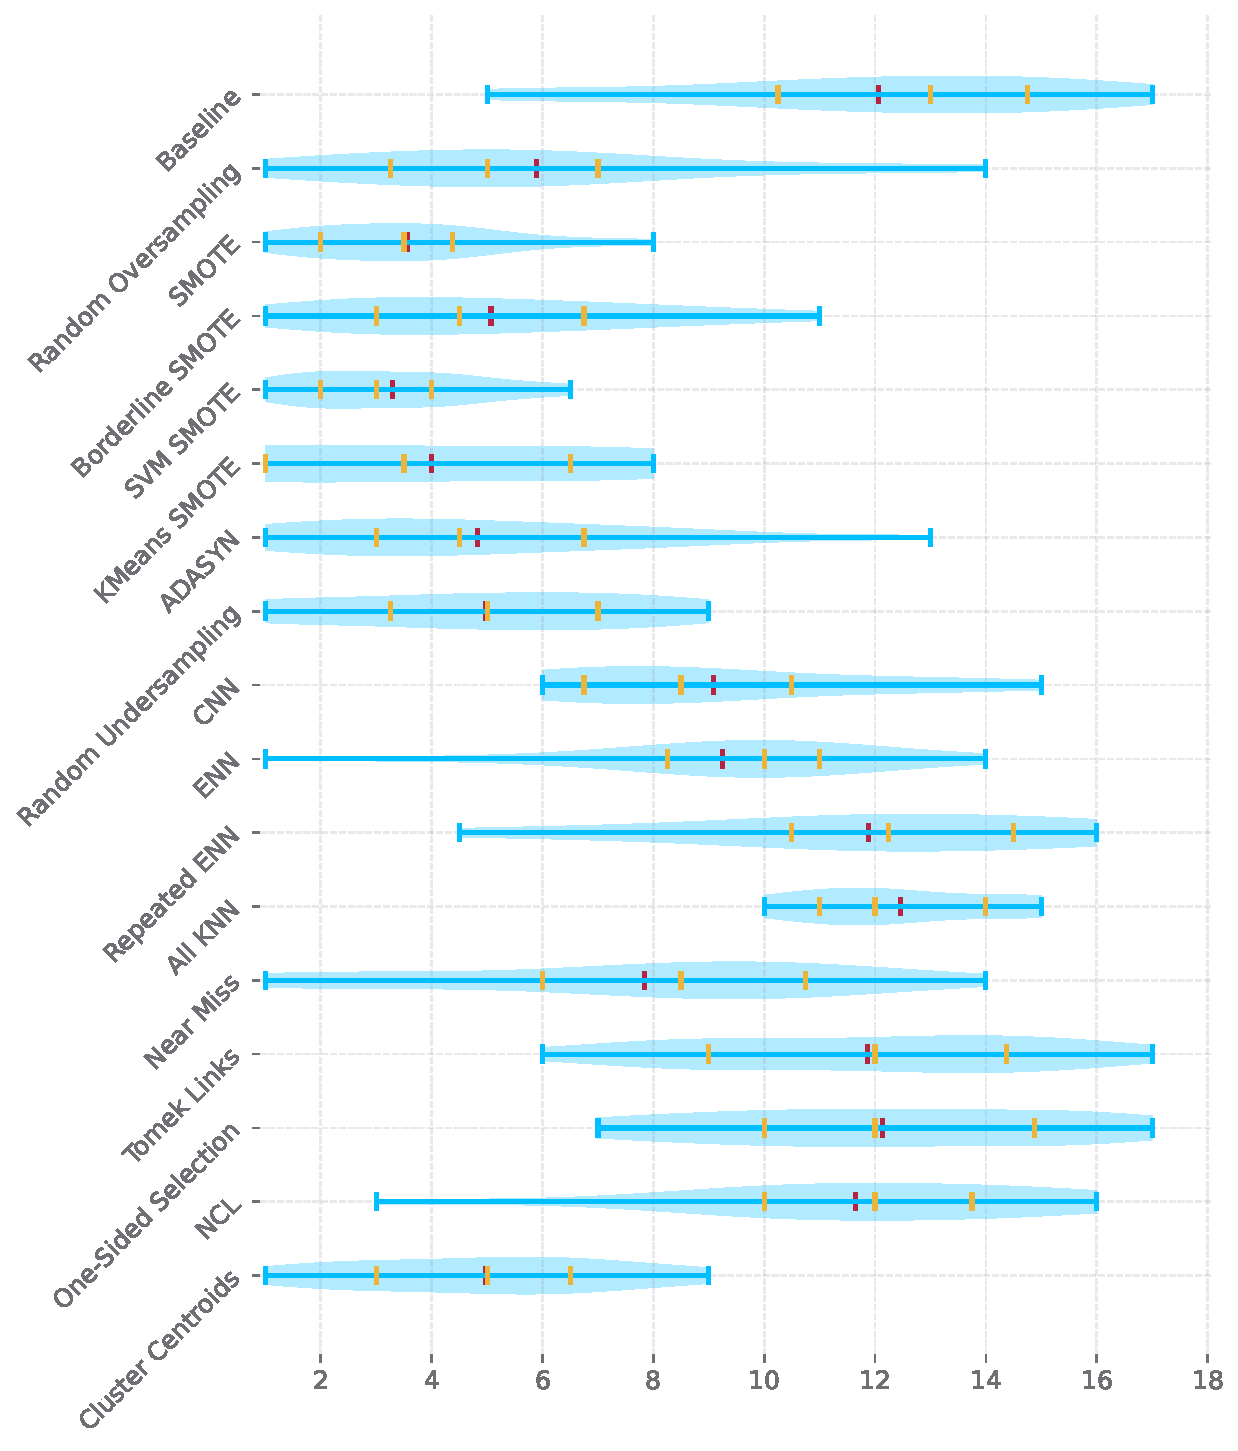
\includegraphics[width=\linewidth]{
            ../thesis/figures/partial_roc_auc_ranks_distribution.pdf
        }
    \end{center}

    The distribution of ranks was computed across all datasets in the experiments. Ranks were
    calculated for each dataset as follows: the highest score is assigned a rank of 1, the
    second-highest a rank of 2 and so on. Average ranks are given in the case of ties. Ranks were
    computed from Partial ROC AUC scores for each preprocessing method separately.
\end{posterbox}


% Right column
\begin{posterbox}[column=1, name=result-times]{Distribution of Preprocessing Times}
    \begin{center}
        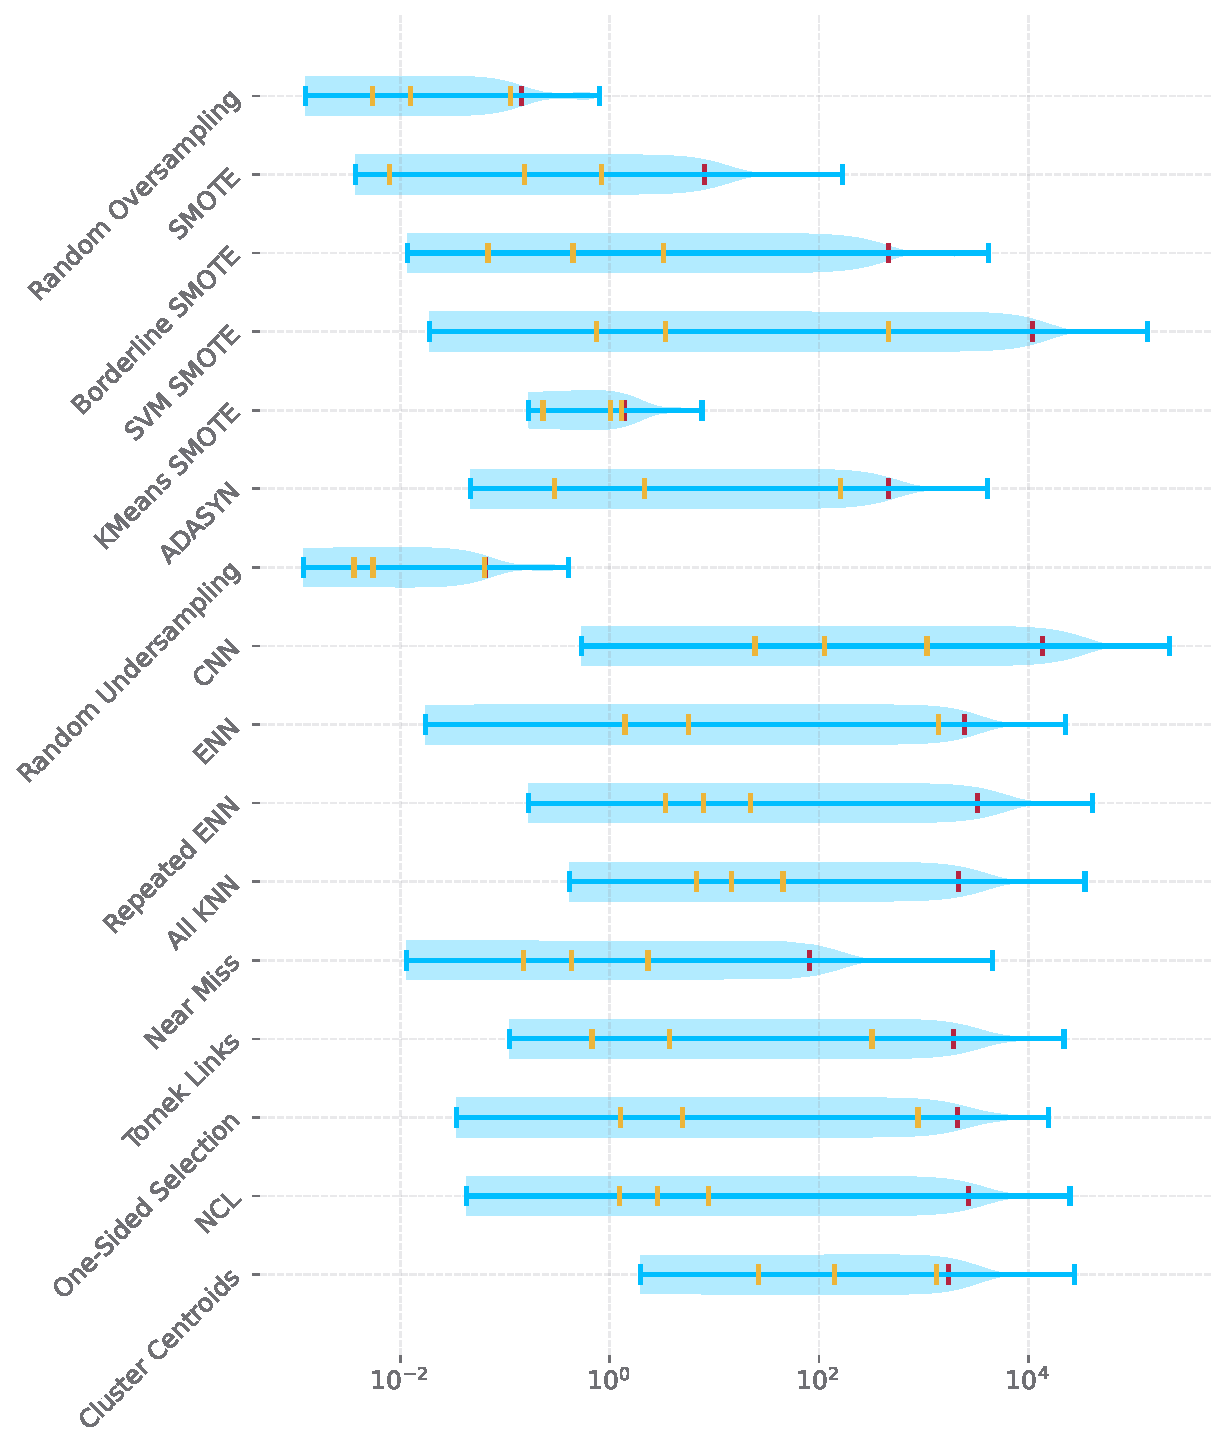
\includegraphics[width=\linewidth]{../thesis/figures/preprocessing_times.pdf}
    \end{center}

    The distribution of preprocessing times in seconds was computed across all datasets in the
    experiment.
\end{posterbox}


\begin{posterbox}[
    column=1, name=result-main, below=result-times,
    headerColorOne=green!50!yellow, boxColorOne=green!10
]{Main results}
    \begin{itemize}[leftmargin=1.2em]
        \item we rejected the null hypothesis that all preprocessing methods have the same
            predictive performance at a 0.001 significance level under all eight evaluation metrics
        \item the results showed a considerable difference in predictive performance between
            oversampling and undersampling methods
        \item the oversampling methods were a bit faster than the undersampling methods, although
            the differences were not significant
    \end{itemize}
\end{posterbox}


\begin{posterbox}[
    column=1, name=conclusion, below=result-main, bottomaligned=result-ranks
]{Conclusion}
    \begin{itemize}[leftmargin=1.2em]
        \item successfully ran a large-scale experiment covering sixteen preprocessing methods over
            eighteen datasets and reported scores in eight evaluation metrics
        \item the source code with instructions for reproduction is available on GitHub in the
            repository Rattko/Bachelor-Thesis
    \end{itemize}

    Future work:
    \begin{itemize}[leftmargin=1.2em]
        \item experiment with combinations of oversampling and undersampling methods
        \item experiment with larger and more skewed datasets from cyber security domains
    \end{itemize}
\end{posterbox}

\end{poster}
\end{document}
